\documentclass{article}
\usepackage{tikz}
\usetikzlibrary{arrows.meta,positioning,calc,shapes.geometric}
\pagestyle{empty}
\begin{document}
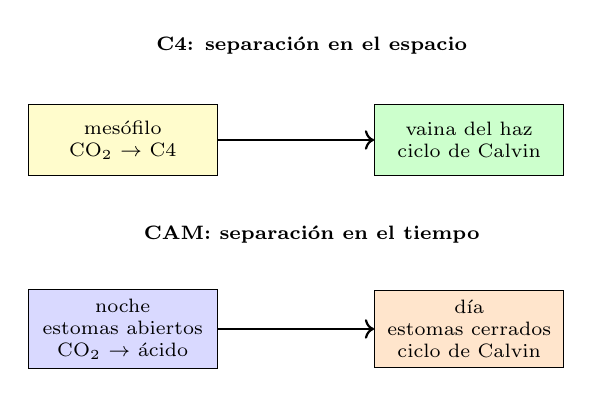
\begin{tikzpicture}
\tikzset{every node/.append style={align=center}}

\node[font=\bfseries\scriptsize] at (3.0,4.2) {C4: separación en el espacio};
\node[draw, fill=yellow!20, minimum width=2.4cm, minimum height=0.9cm, font=\scriptsize] (m) at (0.6,3.0) {mesófilo\\ CO$_2$ $\to$ C4};
\node[draw, fill=green!20, minimum width=2.4cm, minimum height=0.9cm, font=\scriptsize] (v) at (5.0,3.0) {vaina del haz\\ ciclo de Calvin};
\draw[->, thick] (m) -- (v);
\node[font=\bfseries\scriptsize] at (3.0,1.8) {CAM: separación en el tiempo};
\node[draw, fill=blue!15, minimum width=2.4cm, minimum height=0.9cm, font=\scriptsize] (n) at (0.6,0.6) {noche\\ estomas abiertos\\ CO$_2$ $\to$ ácido};
\node[draw, fill=orange!20, minimum width=2.4cm, minimum height=0.9cm, font=\scriptsize] (d) at (5.0,0.6) {día\\ estomas cerrados\\ ciclo de Calvin};
\draw[->, thick] (n) -- (d);

\end{tikzpicture}
\end{document}
